\documentclass[a4paper,11pt]{article}
\usepackage{listingsutf8}
\usepackage{color}
\usepackage{scalefnt}
\usepackage{cancel}
\usepackage{picinpar}
\usepackage{subfig}
\usepackage{graphicx}
\usepackage{amssymb}
\usepackage{amsmath}
\usepackage[brazilian]{babel}
\usepackage[utf8]{inputenc}
\usepackage[T1]{fontenc}
\usepackage{setspace}
\usepackage{caption}
\usepackage[left=2.5cm,right=2.5cm,top=2.0cm,bottom=1.5cm]{geometry}
\usepackage{siunitx}
\usepackage[colorlinks=true,linkcolor=black,linktoc=all, urlcolor=black]{hyperref}
\usepackage{indentfirst}
\usepackage[nottoc]{tocbibind}
\usepackage[fixlanguage]{babelbib}
\selectbiblanguage{brazilian}
\renewcommand{\lstlistingname}{Código}
\lstset{
    inputencoding=utf8,
    extendedchars=true,
    numbers=left,
    numberstyle=\tiny,
    frame=lines,
    captionpos=b,
    literate=
        {á}{{\'a}}1 {é}{{\'e}}1 {í}{{\'i}}1 {ó}{{\'o}}1 {ú}{{\'u}}1 {ù}{{\`u}}1%
        {Á}{{\'A}}1 {É}{{\'E}}1 {Í}{{\'I}}1 {Ó}{{\'O}}1 {Ú}{{\'U}}1%
        {à}{{\`a}}1 {è}{{\'e}}1 {ì}{{\`i}}1 {ò}{{\`o}}1 {ò}{{\`o}}1%
        {À}{{\`A}}1 {È}{{\'E}}1 {Ì}{{\`I}}1 {Ò}{{\`O}}1 {Ò}{{\`O}}1%
        {ä}{{\"a}}1 {ë}{{\"e}}1 {ï}{{\"i}}1 {ö}{{\"o}}1 {ü}{{\"u}}1%
        {Ä}{{\"A}}1 {Ë}{{\"E}}1 {Ï}{{\"I}}1 {Ö}{{\"O}}1 {Ü}{{\"U}}1%
        {â}{{\^a}}1 {ê}{{\^e}}1 {î}{{\^i}}1 {ô}{{\^o}}1 {û}{{\^u}}1%
        {Â}{{\^A}}1 {Ê}{{\^E}}1 {Î}{{\^I}}1 {Ô}{{\^O}}1 {Û}{{\^U}}1%
        {ã}{{\~a}}1 {ẽ}{{\~e}}1 {ĩ}{{\~i}}1 {õ}{{\~o}}1 {ũ}{{\~u}}1%
        {Ã}{{\~A}}1 {Ẽ}{{\~E}}1 {Ĩ}{{\~I}}1 {Õ}{{\~O}}1 {Ũ}{{\~U}}1%
        {œ}{{\oe}}1 {Œ}{{\OE}}1 {æ}{{\ae}}1 {Æ}{{\AE}}1 {ß}{{\ss}}1%
        {ç}{{\c c}}1 {Ç}{{\c C}}1 {ø}{{\o}}1 {å}{{\r a}}1 {Å}{{\r A}}1%
        {€}{{\EUR}}1 {£}{{\pounds}}1,
}

\date{}
\title{
    Uma Ferramenta de Software para a Predição de Desempenho de Workflows Científicos
}

\author{
    Aluno: Lucas Magno \\
    Bolsista PIBIC da CNPq \\
    Instituto de Física (IF) \\
    \\
    Orientadora: Kelly Rosa Braghetto\\
    Departamento de Ciência da Computação (DCC) \\
    Instituto de Matemática e Estatística (IME) \\
    \\
    Universidade de São Paulo \\
    \href{mailto:lucas.magno@usp.br}{lucas.magno@usp.br}
}

\begin{document}
    \maketitle
    \section*{Resumo}
    Este documento descreve as atividades realizadas durante o período de julho de 2013 a junho de 2014 no âmbito do projeto de iniciação científica do aluno Lucas Magno, número USP 7994983, orientado pela Profa. Dra. Kelly Rosa Braghetto e financiado por uma bolsa PIBIC/CNPq.

    O objetivo principal do projeto foi desenvolver uma ferramenta de software para a conversão automática de modelos de \emph{workflows} em modelos estocásticos na álgebra de processos \emph{PEPA - Performance Evaluation Process Algebra} \cite{web:pepa} . A partir desses modelos estocásticos, é possível extrair predições de desempenho de \emph{workflows}.
    \section*{Abstract}

    \newpage
    \section*{Introdução}
        Inicialmente desenvolvidos para automatizar processos industriais e empresariais, os \emph{workflows} se popularizaram e passaram a ser usados na modelagem e automatização de experimentos científicos em diversas áreas da ciência. Um \emph{workflow científico} é a descrição completa ou parcial de um experimento científico em termo de suas atividades, controles de fluxo e dependência de dados \cite{phd:gadelha12}.

        Há várias maneiras de se representar um \emph{workflow científico}, entre elas \emph{grafos direcionados}, \emph{UML \emph{(Unified Modeling Language)}}, \emph{redes de Petri} e \emph{álgebras de processo} \cite{phd:oga11}:. Estes mecanismos de representação são usados para criar modelos que especificam a ordem de execução das atividades dos \emph{workflows}. Além disso, as redes de Petri e as álgebras de processo são linguagens formais, permitindo que se verifiquem propriedades qualitativas e quantitativas dos modelos de \emph{workflow}. Neste trabalho, no entando, somente foram utilizados grafos direcionados e álgebras de processo.

    Para simplificar sua implementação, considera-se que \emph{workflows} sejam compostos por \emph{atividades}, que representam atividades reais de um experimento, e estruturas para descrever o fluxo de controle, como \emph{sequência}, \emph{paralelismo}, \emph{escolha} e \emph{sincronização}, definidas por meio dos operadores \emph{AND} (paralelismo/sincronização), \emph{XOR} (escolha exclusiva/junção) e \emph{OR} (escolha múltipla/junção).

        Por ser comum em experimentos científicos a manipulação de de enormes quantidades de dados e a presença de processos muito demorados, é necessária a análise do desempenho dos \emph{workflows} associados, que pode ser feita através de \emph{medição}, \emph{simulação} ou \emph{modelagem analítica} \cite{phd:kelly11}. Foi escolhida, então, a modelagem analítica, um método preditivo e rápido, implementada por meio de uma álgebra de processos estocástica, a \emph{PEPA}, pois seu uso ainda não foi profundamente explorado para a análise de desempenho preditiva de \emph{workflows} científicos.

    \section*{Objetivos}

        Uma desvantagem da modelagem analítica usando \emph{PEPA} é a necessidade da descrição do \emph{workflow} em uma linguagem de modelagem estocástica e utilização de programas específicos para a análise, exigindo do usuário um certo nível de conhecimento sobre álgebras de processo. No entanto, \emph{workflows} científicos são utilizados em diversas áreas da ciência que não necessitam de um grande aprofundamento em computação, o que pode inviabilizar a aplicação deste método.

        O objetivo do trabalho foi facilitar a extração de predições de desempenho para \emph{workflows} científicos. Para isso, foi desenvolvida uma ferramenta de software que gera modelos estocásticos em \emph{PEPA} e sua solução numérica a partir de modelos de \emph{workflows}.

        Os modelos de \emph{workflows} usados como entrada para a ferramenta são descritos textualmente na forma de um grafo dirigido - uma representação simples e que pode ser usada com facilidade por usuários não especialistas. Além do modelo em \emph{PEPA} e sua solução, a ferramenta também gera uma representação gráfica do modelo de \emph{workflow}, que permite que o usuário possa verificá-lo mais facilmente.

    \section*{Materiais e Métodos}
        Para que possua um modelo correspondente em \emph{PEPA}, um modelo de \emph{workflow} precisa ser bem estruturado e não possuir ambiguidades semânticas. Por essa razão, neste trabalho consideramos apenas modelos de \emph{workflow} que apresentam somente um ponto de entrada e um ponto de saída, têm sua estrutura em forma de ``blocos''  e não apresentam ciclos, ou laços, o que permite uma implementação mais simples.

        Para automatizar o processo de predição de desempenho, foi implementado um programa na linguagem \emph{Python} (versão 2.7), por flexibilidade, facilidade de aprendizado e grande número de bibliotecas auxiliares. Seu código fonte, detalhes de sua execução, dependências e exemplos de \emph{workflow} de entrada e suas representações em \emph{PEPA} geradas podem ser conferidos na página do projeto \cite{web:script}.

        \newpage
        O programa pode ser resumido nas seguintes etapas:

        \begin{enumerate}
            \item Lê como entrada uma descrição textual de um \emph{workflow} em uma gramática simples baseada na linguagem \emph{DOT} \cite{web:dot} através dos analisadores léxico e sintático gerados a partir da biblioteca \emph{PLY}, \emph{Python Lex-Yacc} \cite{web:ply}.
            \item Gera uma estrutura de dados baseada em grafo na memória representando o \emph{workflow} através de classes explicitamente definidas que permitem a manipulação de nós, arestas e \emph{workflows}.
            \item Gera uma uma descrição do \emph{workflow} de entrada em linguagem \emph{DOT} e sua visualização através da biblioteca \emph{Graphviz} \cite{web:graphviz}.
            \item Gera um modelo analítico do \emph{workflow} em \emph{PEPA}
            \item Gera a solução numérica do modelo analítico e extrai seus índices de desempenho através da biblioteca \emph{pyPEPA} \cite{web:pypepa}, uma implementação recente da \emph{PEPA} em \emph{Python}.
        \end{enumerate}

    \section*{Resultados}

        Ao processar um \emph{workflow}, então, o programa cria arquivos de saída contendo a descrição do \emph{workflow} em \emph{DOT}, sua visualização, sua descrição em \emph{PEPA} e os índices de desempenho dela extraídos. Estes arquivos, entretanto, são geralmente muito extensos, então serão mostrados aqui somente um exemplo de \emph{workflow} de entrada e sua visualização. Demais exemplos estão disponíveis na página do projeto.\\

        \begin{minipage}[c]{0.6\textwidth}
            \centering
            \lstinputlisting[caption={Exemplo de descrição do \emph{workflow} de entrada},label=lst:dot,tabsize=2]{example}
        \end{minipage}%
        \begin{minipage}[r]{0.4\textwidth}
            \centering
            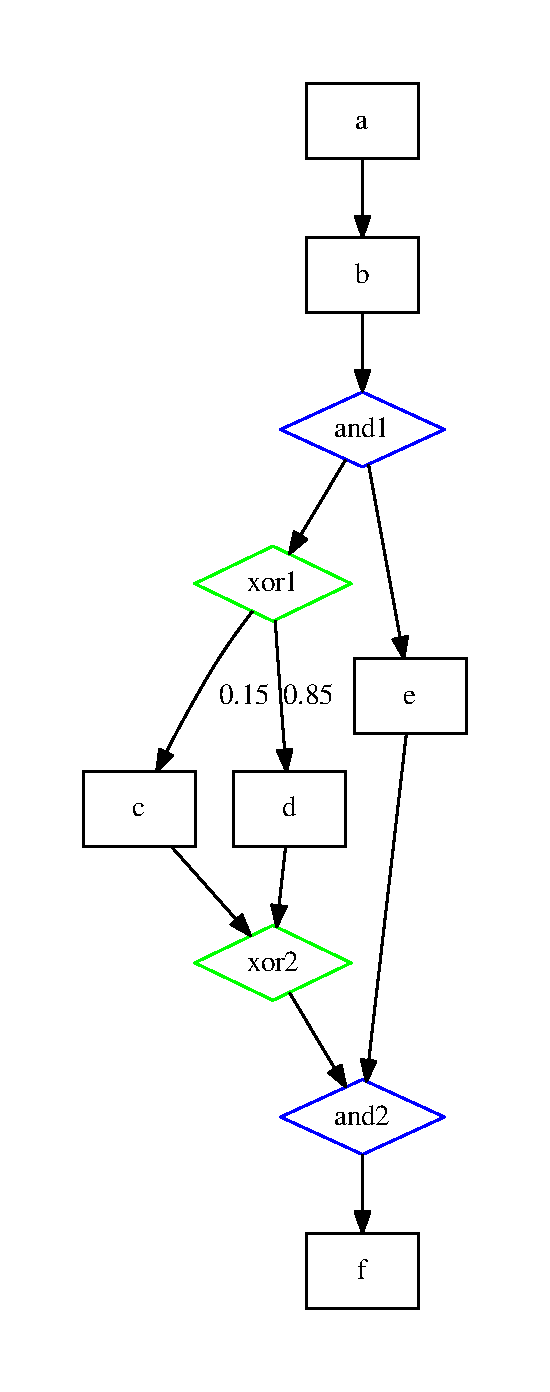
\includegraphics[width=0.65\linewidth]{example.pdf}
            \captionof{figure}{Exemplo de visualização do \emph{workflow} criada a partir do código em DOT}
            \label{fig:pdf}
        \end{minipage}
    \newpage
    \section*{Conclusões}

        Neste projeto de iniciação científica, foi desenvolvida uma ferramenta de software que converte de forma automática modelos de \emph{workflow} em modelos estocásticos e, a partir destes últimos, extrai medidas de desempenho dos \emph{workflows}, facilitando o uso de ferramentas de predição por usuários não-especialistas.

        Os modelos de \emph{workflow} recebidos como entrada para o programa são definidos por meio de uma notação simples que permite descrever os modelos mais comuns de experimentos científicos.

        Para a geração dos modelos estocásticos, usou-se a linguagem \emph{PEPA}, capaz de descrever uma grande variedade de processos, embora tenha uma sintaxe complexa. A análise numérica desses modelos foi feita por meio da biblioteca \emph{pyPEPA}, uma implementação recente de \emph{PEPA} em \emph{Python}.

        A escolha de \emph{Python} como linguagem de implementação do programa se provou bastante favorável, já que as estruturas de dados e bibliotecas existentes nessa linguagem agilizaram o desenvolvimento das funcionalidades primárias do programa.

        A complexidade da sintaxe da PEPA, entretanto, dificultou a conversão dos modelos de workflow, pois exigiu o tratamento de diversas especificidades desta. Além disso, a implementação recente da pyPEPA apresentou diversos obstáculos durante o projeto, como sua sintaxe muito restritiva (ela ainda não suporta completamente a sintaxe da PEPA) e sua documentação escassa.

        Por estes motivos, as etapas relativas a essas ferramentas ocuparam grande parte do cronograma do projeto, não sendo possível, portanto, realizar outras funcionalidades inicialmente sugeridas neste trabalho, mas que ainda são interessantes de se implementar, como por exemplo:
        \begin{itemize}
            \item Gerar modelos analíticos de \emph{workflows} que contenham o operador \emph{OR}
            \item Definição de uma linguagem para descrição dos recursos que podem ser utilizados por um \emph{workflow}
            \item Incorporação de informações sobre recursos nos modelos analíticos
            \item Permitir a descrição de \emph{workflows} cuja estrutura não seja ``em blocos''
        \end{itemize}

    \bibliographystyle{bababbr3}
    \bibliography{references}

\end{document}
